\section{Aplicación de ejemplo}

Para comprender mejor esta problemática veamos un ejemplo. Supongamos una simple
aplicación, donde los clientes de un banco pueden transferir dinero de
una cuenta a otra. Al realizar una transferencia, hay que extraer el monto
indicado de una cuenta, y depositarlo en otra. 
Al ejecutar cualquiera de estas dos operaciones se pueden producir errores,
como por ejemplo, que no haya saldo saldo suficiente, o que el depósito supere
el máximo permitido.
La  figura \ref{example} muestra el diagrama de clases de la aplicación de
ejemplo

\medskip
	\begin{figure}[h]
		\centering
		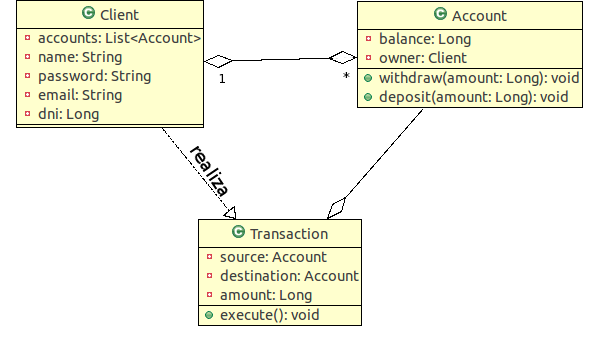
\includegraphics[width=250px, height=150px]{img/transaccion}
		\caption{Diagrama UML de la aplicación de ejemplo}
		\label{example}
	\end{figure}	


El sistema me permite realizar múltiples transferencias a la vez y por último
realizar la confirmación o la cancelación de todas ellas. También brinda la posibilidad
de realizar múltiples transacciones, por ejemplo, en la edición de un cliente,
se puede editar, eliminar o crear cuentas. A su vez se puede hacer una
transferencia a otra cuenta. En cada una de esas operaciones se esta
trabajando en dentro de una transacción. y las operaciones pueden ser
canceladas por unidad, es decir, se cancelan o se confirman por transacción.


Caso de uso 1: transferir plata.
Tres ventajas:
- queda más simple
- menos posibilidad de mandármela
- concurrencia.

\begin{figure}[h]
	\begin{lstlisting}
		public void execute(){
			this.source.withdraw(this.amount);
			this.destination.deposit(this.amount);
		}
	\end{lstlisting}
	\caption{Fragmento de código de la Clase Transaction}
	\label{executeTransaction}
\end{figure}

Caso de uso 2: transferencias múltiples.
muchas transferencias en una única transacción\ldots fijate si sale algo y si no
lo volamos.